\documentclass[main.tex]{subfiles}

\begin{document}

\section{Aufgabe 3}
In Aufgabe A5 auf Aufgabenblatt Nr. 1 wurden bereits Anwendungsfälle für einen Fahrkartenautomat einer regionalen Privatbahn besprochen. Der Ablauf des Anwendungsfalls »Fahrkartenkauf« soll nun präzisiert werden. Die zugehörigen Aktionen lauten:

\begin{itemize}
\item Verbindung suchen und auswählen
\item Passende Fahrkarte auswählen
\item Optional: Verbindungsdetails ausdrucken lassen
\item Geld einwerfen
\item Fahrkarte entnehmen
\item Ggf. Rückgeld entnehmen
\item Ggf. Verbindungsdetails entnehmen
\end{itemize}

Erst wenn ausreichend Geld eingeworfen wurde, wird die Fahrkarte gedruckt. Bis dahin kann der Fahrkartenkauf jederzeit durch den Benutzer abgebrochen werden. Sollte in diesem Fall bereits Geld eingeworfen worden sein, dann wird es wieder ausgegeben. Der Fahrkartenautomat nimmt nur Bargeld an.
Modellieren Sie den Fahrkartenkauf als UML-Aktivitätsdiagramm aus Sicht der Nutzenden. Modellieren Sie dabei auch die aus Sicht der Nutzenden relevanten Objekte und Objektflüsse.
\textit{Hinweis: den Fall, dass der Fahrkartenautomat eventuell nicht genügend Rückgeld ausgeben kann, können Sie bei der Modellierung ignorieren.}

\pagebreak
\subsection{Lösung 3}
\begin{figure}[h]
    \makebox[\textwidth][c]{
        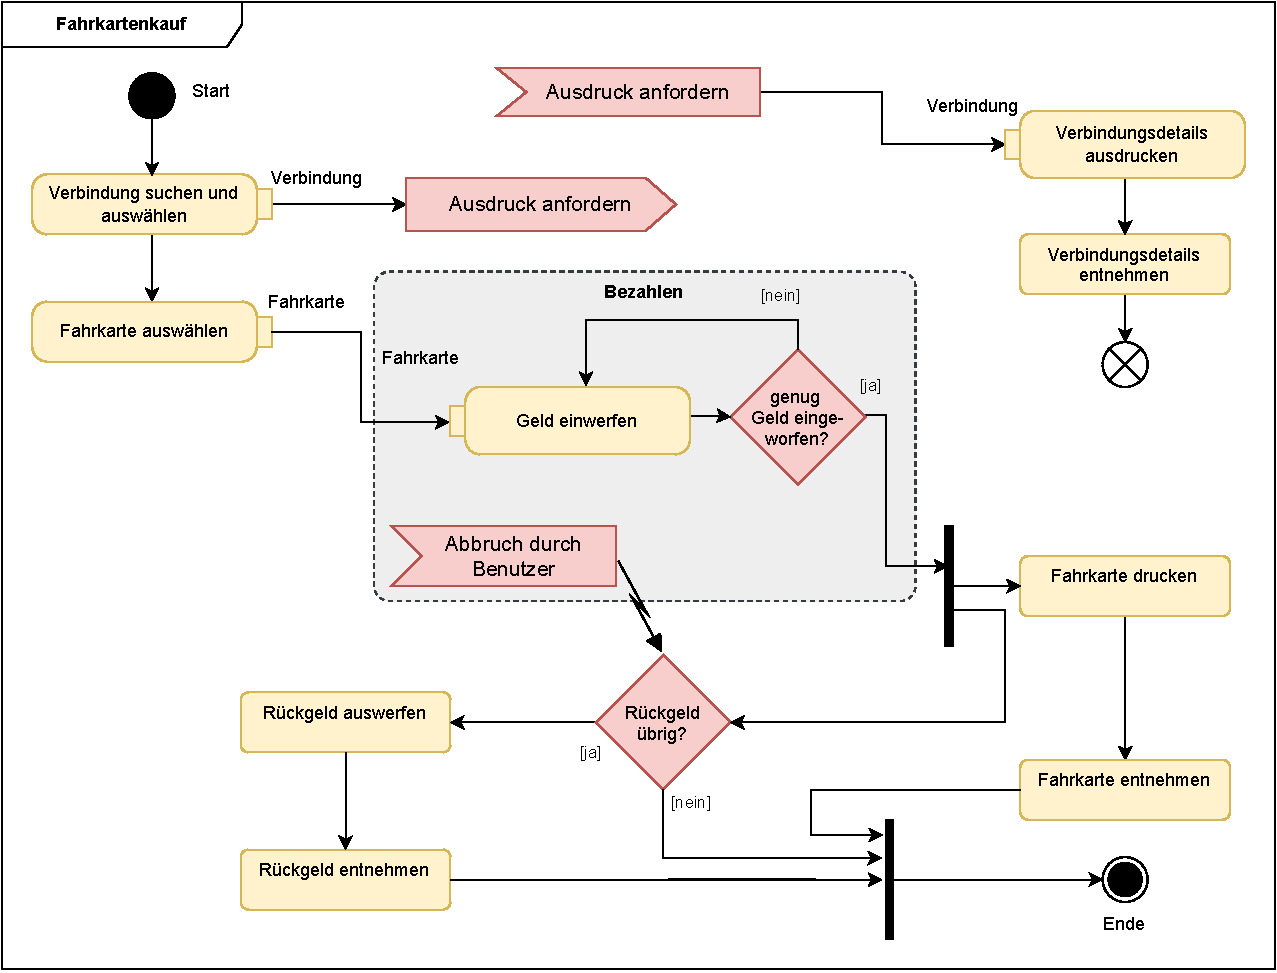
\includegraphics[width=1.2\linewidth]{h03_A3.pdf}
    }
    \caption{Lösung der Aufgabe 3}
    \label{fig:lgs3}
\end{figure}

\end{document}
